%%%%Similar to some other part

The diagram in Figure \ref{fig:systemInteraction} shows the interaction between the subsystems of the ITU-MiniTwit system.

\begin{enumerate}
    \item The code source consists of the react app for our front end, the spring API for the backend, the simulator for testing our endpoints and sending request throughout the course and finally the deployment folder with the vagrantfile for the deployment process.  The developer makes all the relevant configurations to GitHub, Azure, Docker and GitHub Action. From the development machine the code can be push/pull from GitHub.
    \item For the second stage we have the most important git repositories corresponding for the backend, frontend, simulator and deployment. After that we create 3 .yml files named docker-publish.yml for the 3 first repositories named above. Those files get triggered on push.
    \item After getting triggered the GitHub Action CI/CD pipeline automatically builds the docker images and push it to Docker Hub. If the docker images are pushed successfully, another GitHub Action triggers. This action updates the docker containers on the server For details see Appendix \ref{subsec: GithubActionsPipeline}
\end{enumerate}

\begin{figure}[h]
    \centering
    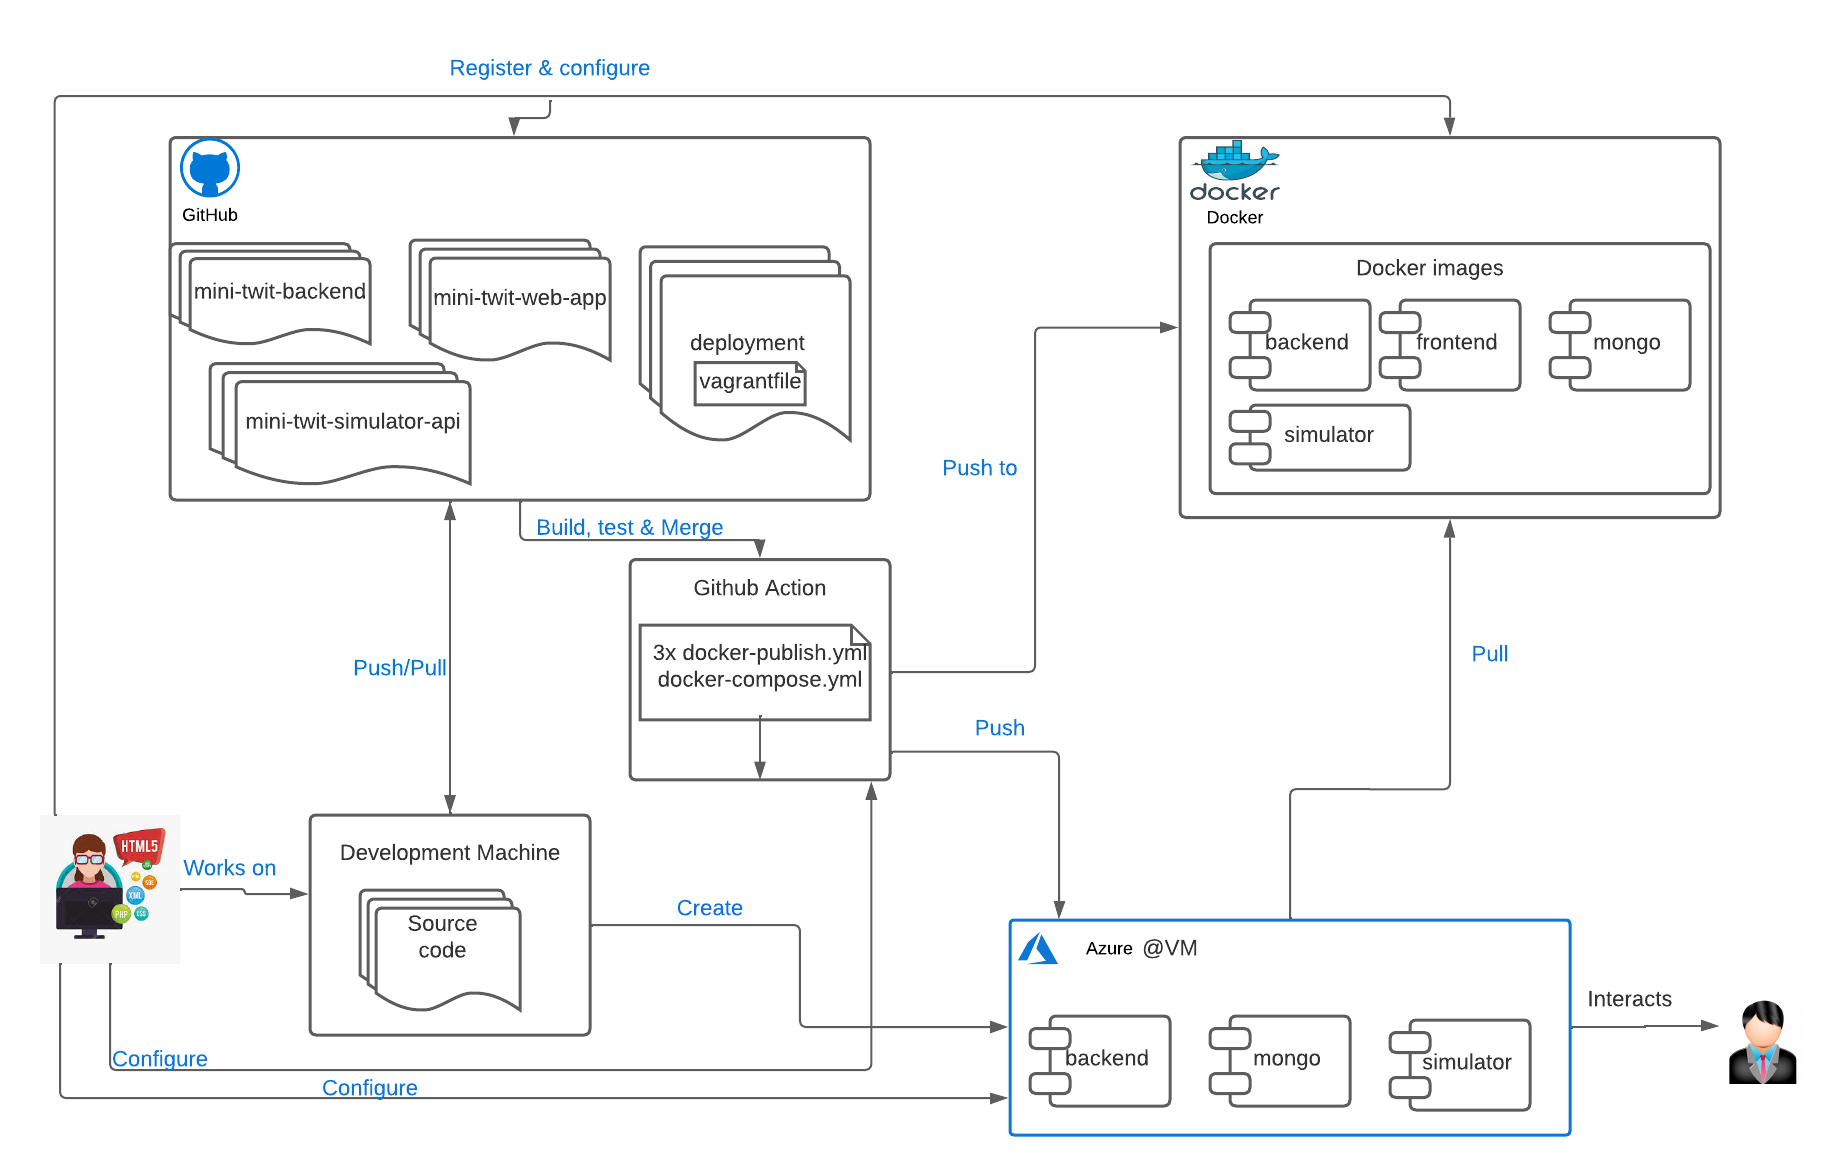
\includegraphics[width = \textwidth]{images/NewSystemInteraction.png}
    \caption{The interactions of the subsystems used in this project}
    \label{fig:systemInteraction}
\end{figure}